\section{Industria: el promedio mejora sin una mejora generalizada}
En la industria manufacturera, el índice ponderado de productividad aumenta en las tres ventanas examinadas: 8,2 puntos logarítmicos en 2010--2015, 10,7 en 2015--2019 y 10,4 en 2019--2024. La contribución de la media sin ponderar de las empresas sobrevivientes es negativa en los tres periodos. En cambio, la covarianza entre productividad y participación en el empleo aumenta y la salida aporta positivamente.

\begin{figure}[H]
\centering
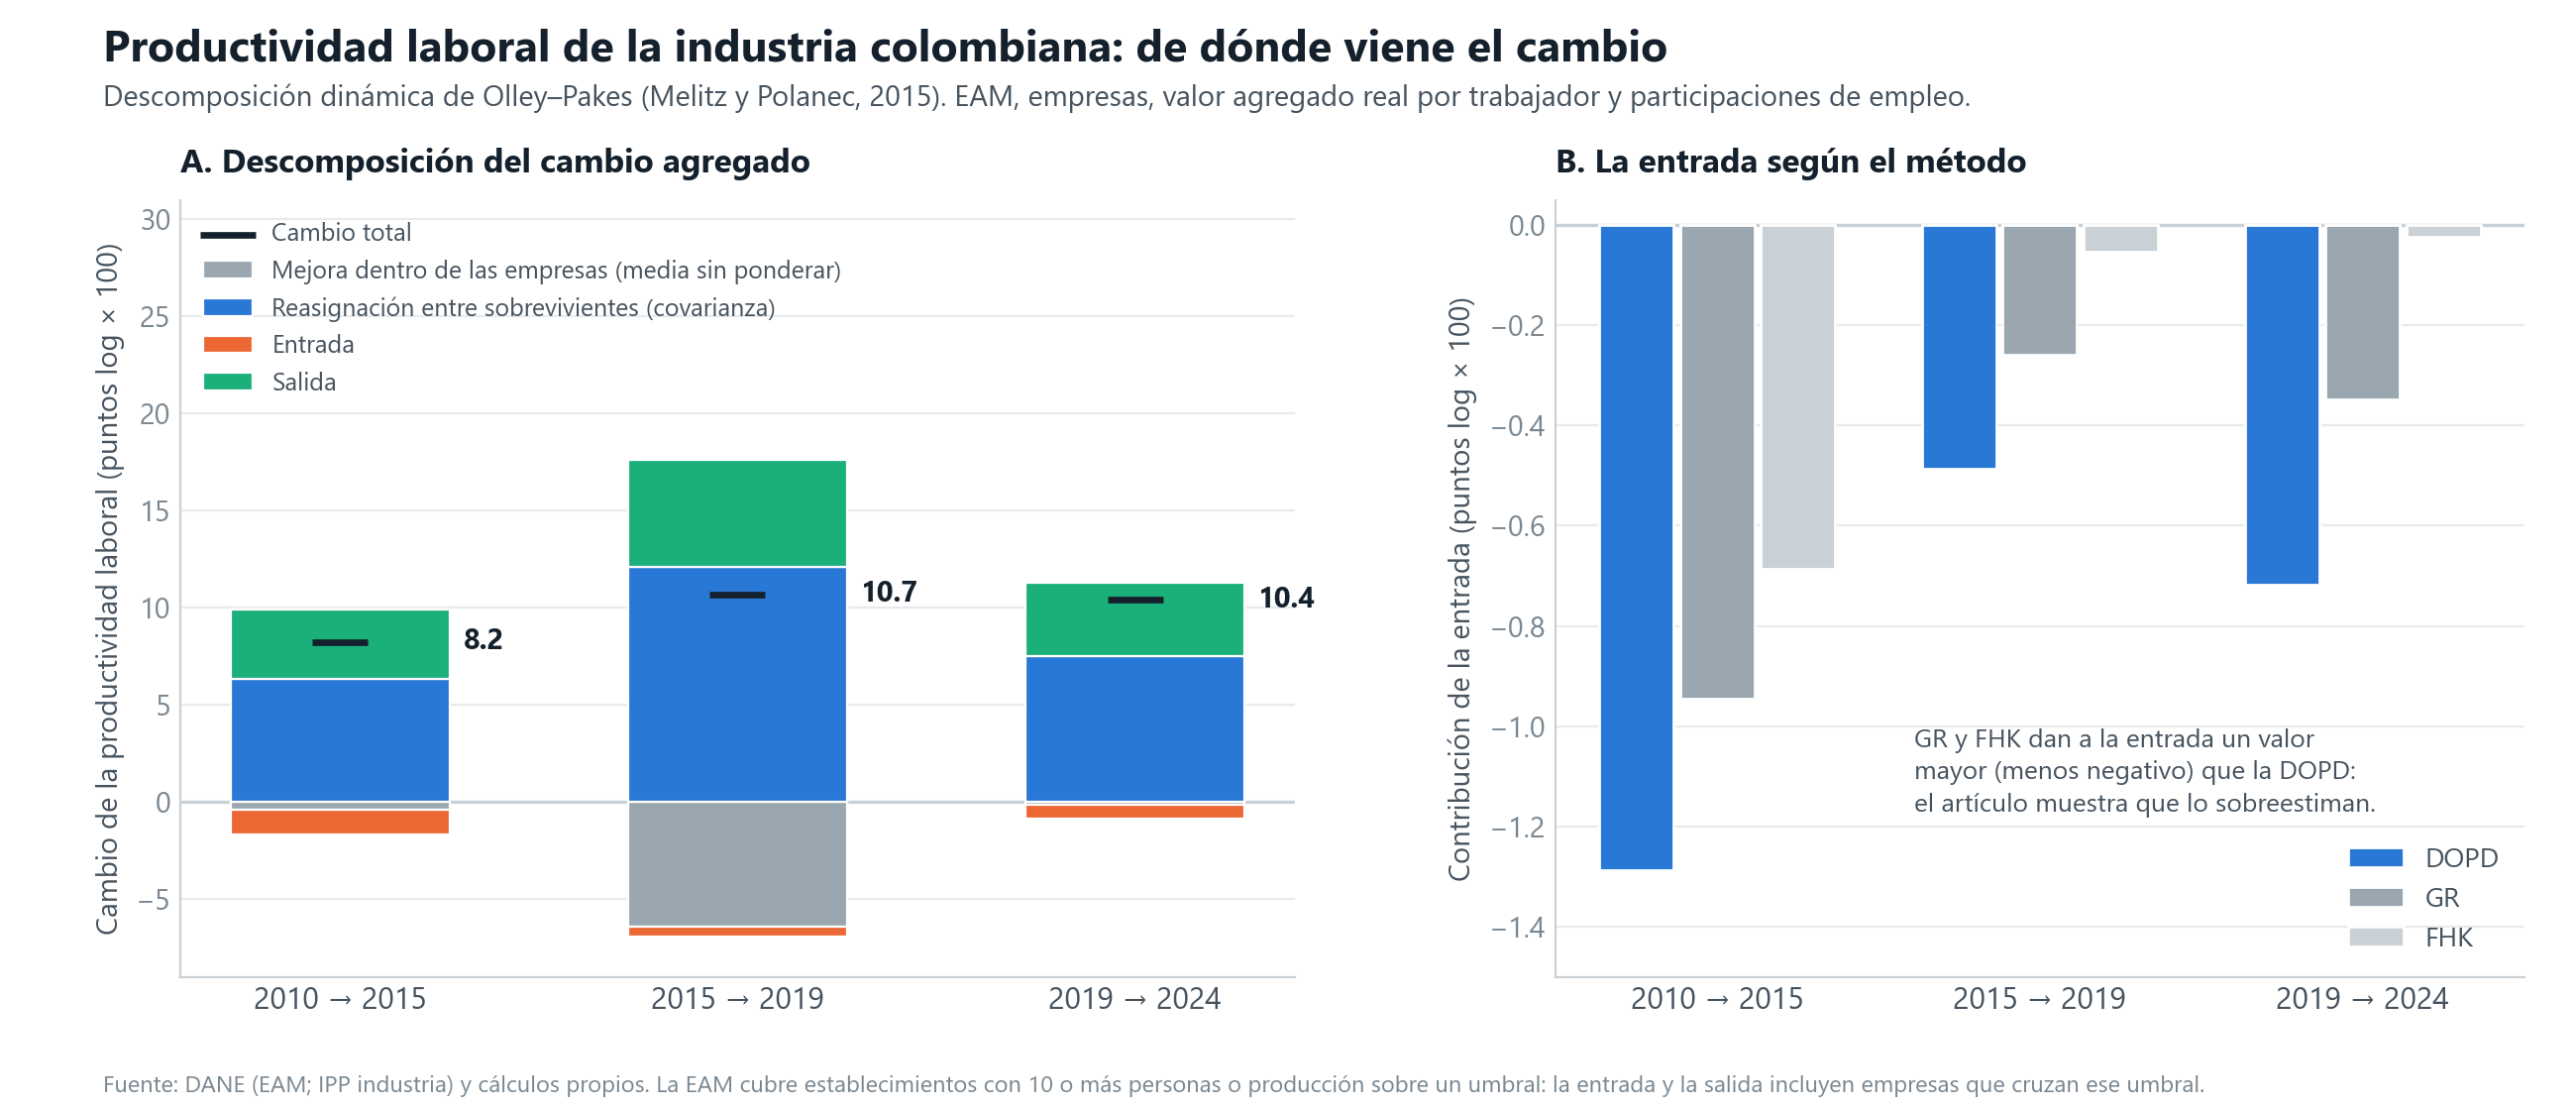
\includegraphics[width=\linewidth]{melitz_polanec/fig_dopd_laboral.png}
\caption{Industria: componentes del cambio y comparación de la entrada}
\label{fig:industria}
\fuente{Fuente: DANE, EAM e IPP; cálculos propios. Participaciones de empleo. Unidades: diferencias del índice de logaritmos, multiplicadas por 100. La marca negra es la suma algebraica de las contribuciones.}
\end{figure}

El periodo 2015--2019 es ilustrativo: el cambio de la media de sobrevivientes resta 6,4 puntos, mientras la covarianza aporta 12,1 y la salida 5,5. El agregado mejora aunque la empresa sobreviviente promedio no lo haga. La covarianza puede variar tanto por cambios de tamaño como por cambios de productividad relativa; no identifica por sí sola flujos de trabajadores entre empresas.

La entrada resta entre 0,5 y 1,3 puntos. En esta descomposición, ello significa que las entrantes tienen menor productividad ponderada que las sobrevivientes del año final. No evalúa sus beneficios futuros ni compara la economía observada con una economía sin nuevas empresas. La contribución positiva de la salida indica que las salientes eran menos productivas que las sobrevivientes del año inicial.

El panel B muestra que las referencias utilizadas por GR y FHK atribuyen a la entrada una contribución menos negativa que DOPD. Es una diferencia contable de método, no una estimación causal. Su magnitud debe revisarse con las pruebas de robustez antes de adoptar una interpretación económica definitiva.
\clearpage
\section{Comercio: recuperación con una discontinuidad de datos}
Entre 2015 y 2019, el índice de productividad del comercio cae 0,9 puntos logarítmicos. La media de sobrevivientes aporta $-10,9$, compensada en gran parte por la covarianza ($+7,8$) y la salida ($+2,7$). Entre 2020 y 2024, el índice aumenta 8,7 puntos, con aportes positivos de los cuatro componentes.

\begin{figure}[H]
\centering
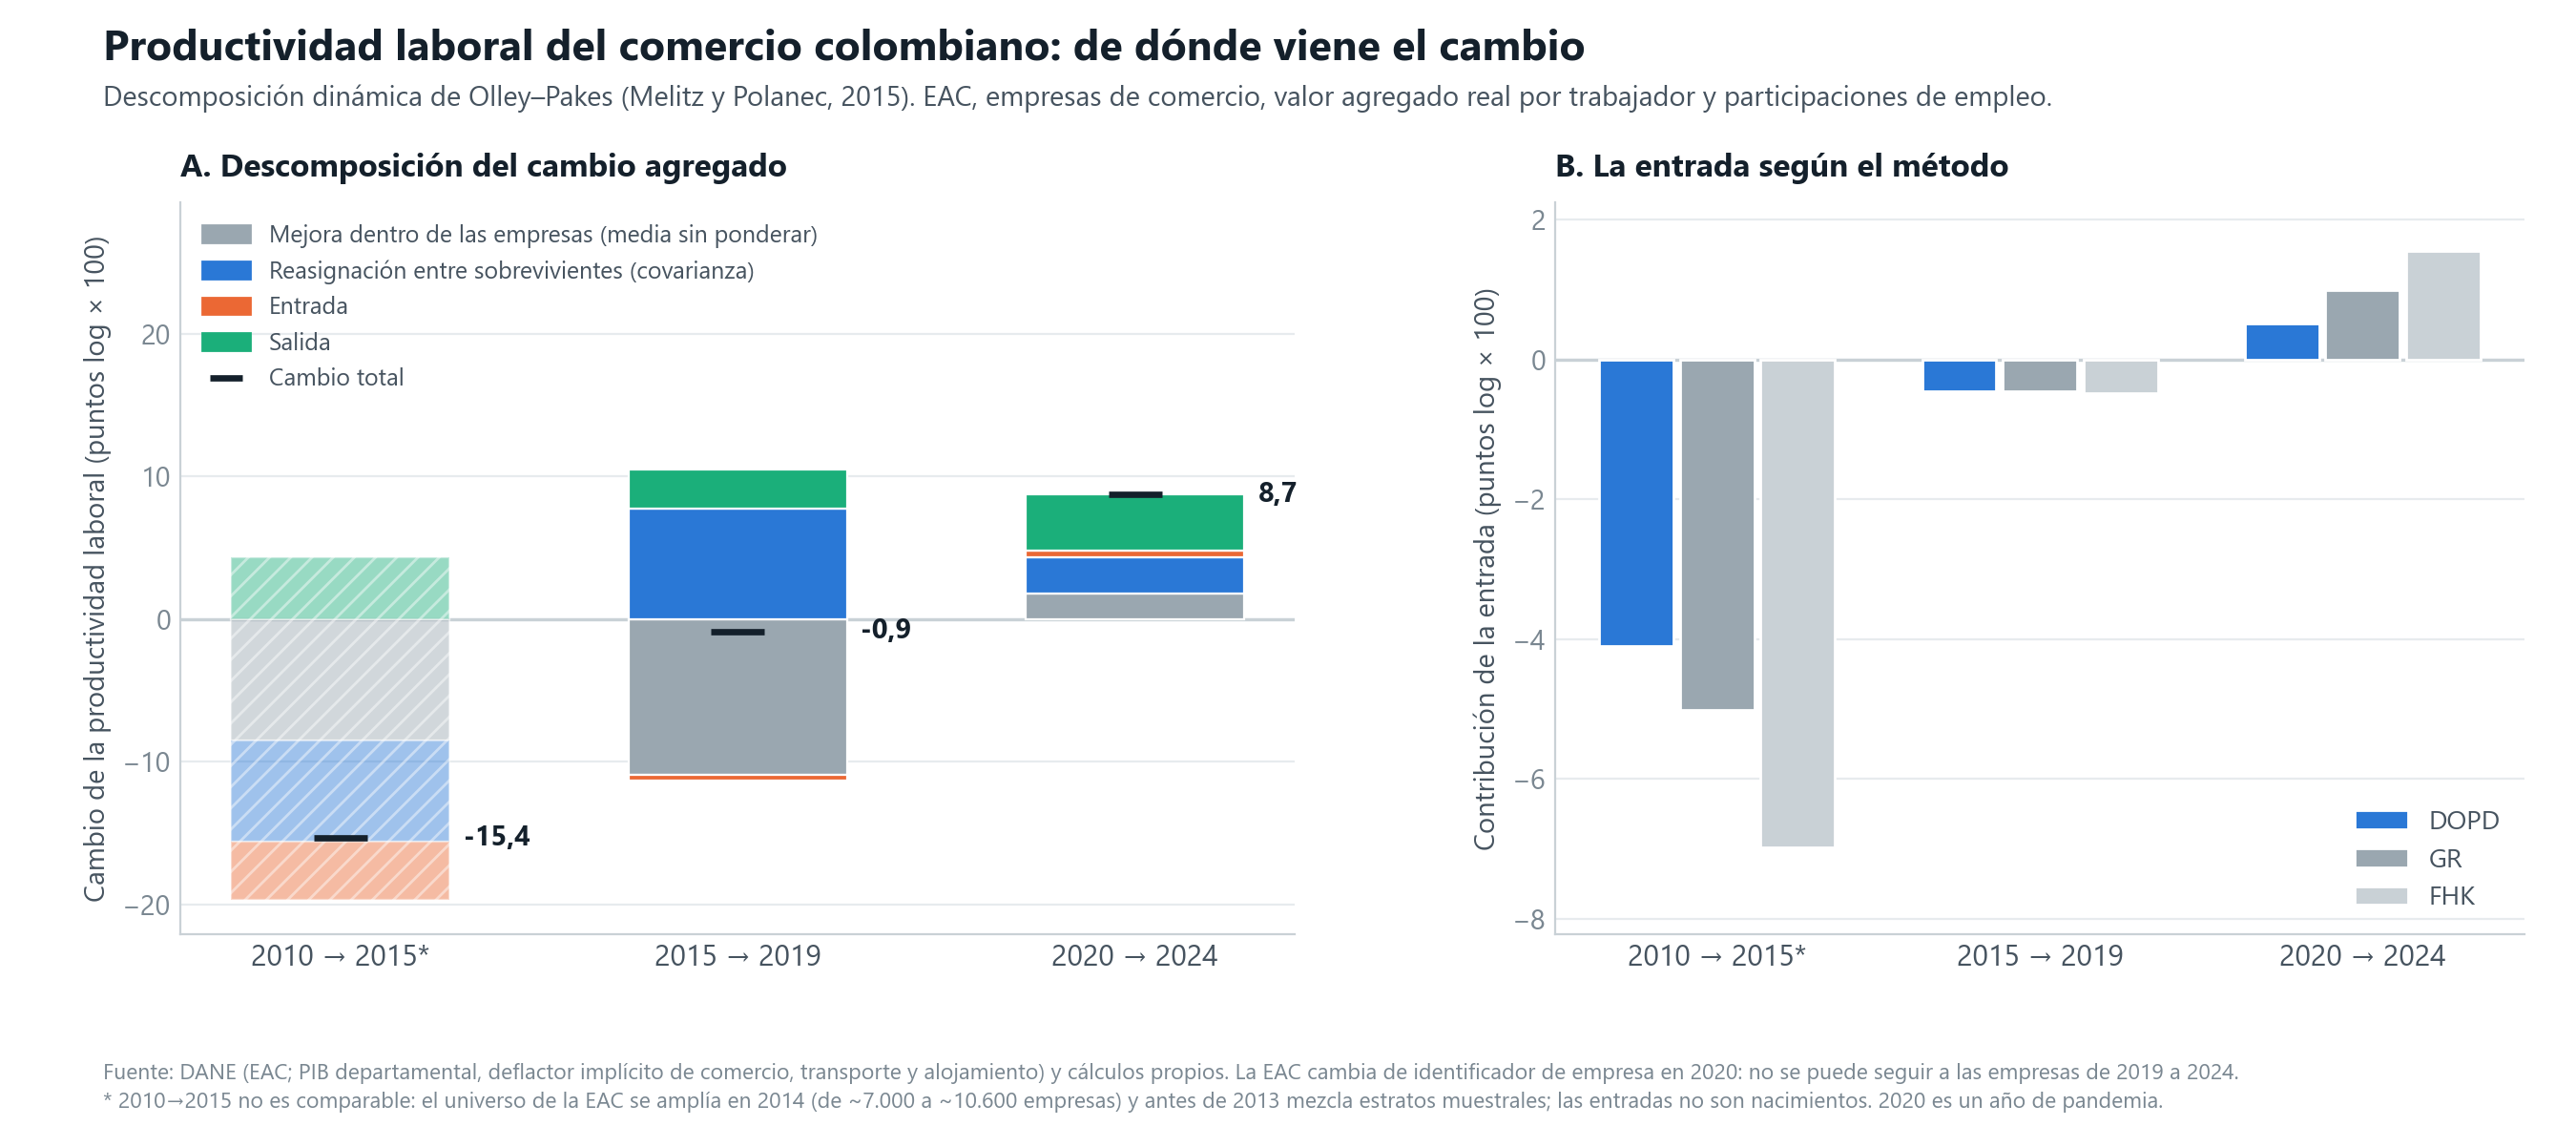
\includegraphics[width=\linewidth]{melitz_polanec/fig_dopd_laboral_EAC.png}
\caption{Comercio: resultados y una ventana de cobertura no comparable}
\fuente{Fuente: DANE, EAC y cuentas departamentales; cálculos propios. La ventana sombreada 2010--2015 no es comparable por cambios de cobertura. La ventana 2020--2024 parte del año de pandemia y no equivale a 2019--2024.}
\end{figure}

El identificador de las empresas cambia entre 2019 y 2020, sin coincidencias que permitan seguirlas directamente. Por esta razón, no se construye una descomposición 2019--2024. Además, la ampliación de cobertura de 2014 impide usar 2010--2015 como evidencia comparable de dinámica empresarial. Estas ventanas se conservan en los archivos de diagnóstico, pero no sustentan las conclusiones principales.

La construcción del panel detectó un intercambio aparente entre las variables de ventas y valor agregado en 2017 y 2018, y aplicó una corrección documentada. Es una decisión de procesamiento que requiere contraste adicional con los archivos y diccionarios originales. El deflactor de comercio también explica parte de la caída del componente de la media; no debe atribuirse toda esa caída a deterioro técnico de las empresas.
\clearpage
\section{Servicios: mejora interna y cambios de composición}
El índice de productividad de servicios aumenta 3,5 puntos logarítmicos en 2010--2015, 6,4 en 2015--2019 y 13,4 en 2019--2024. En los dos primeros periodos, la media sin ponderar de sobrevivientes disminuye. En el último, aporta 8,4 puntos y se suma al aporte positivo de la covarianza ($+6,9$).

\begin{figure}[H]
\centering
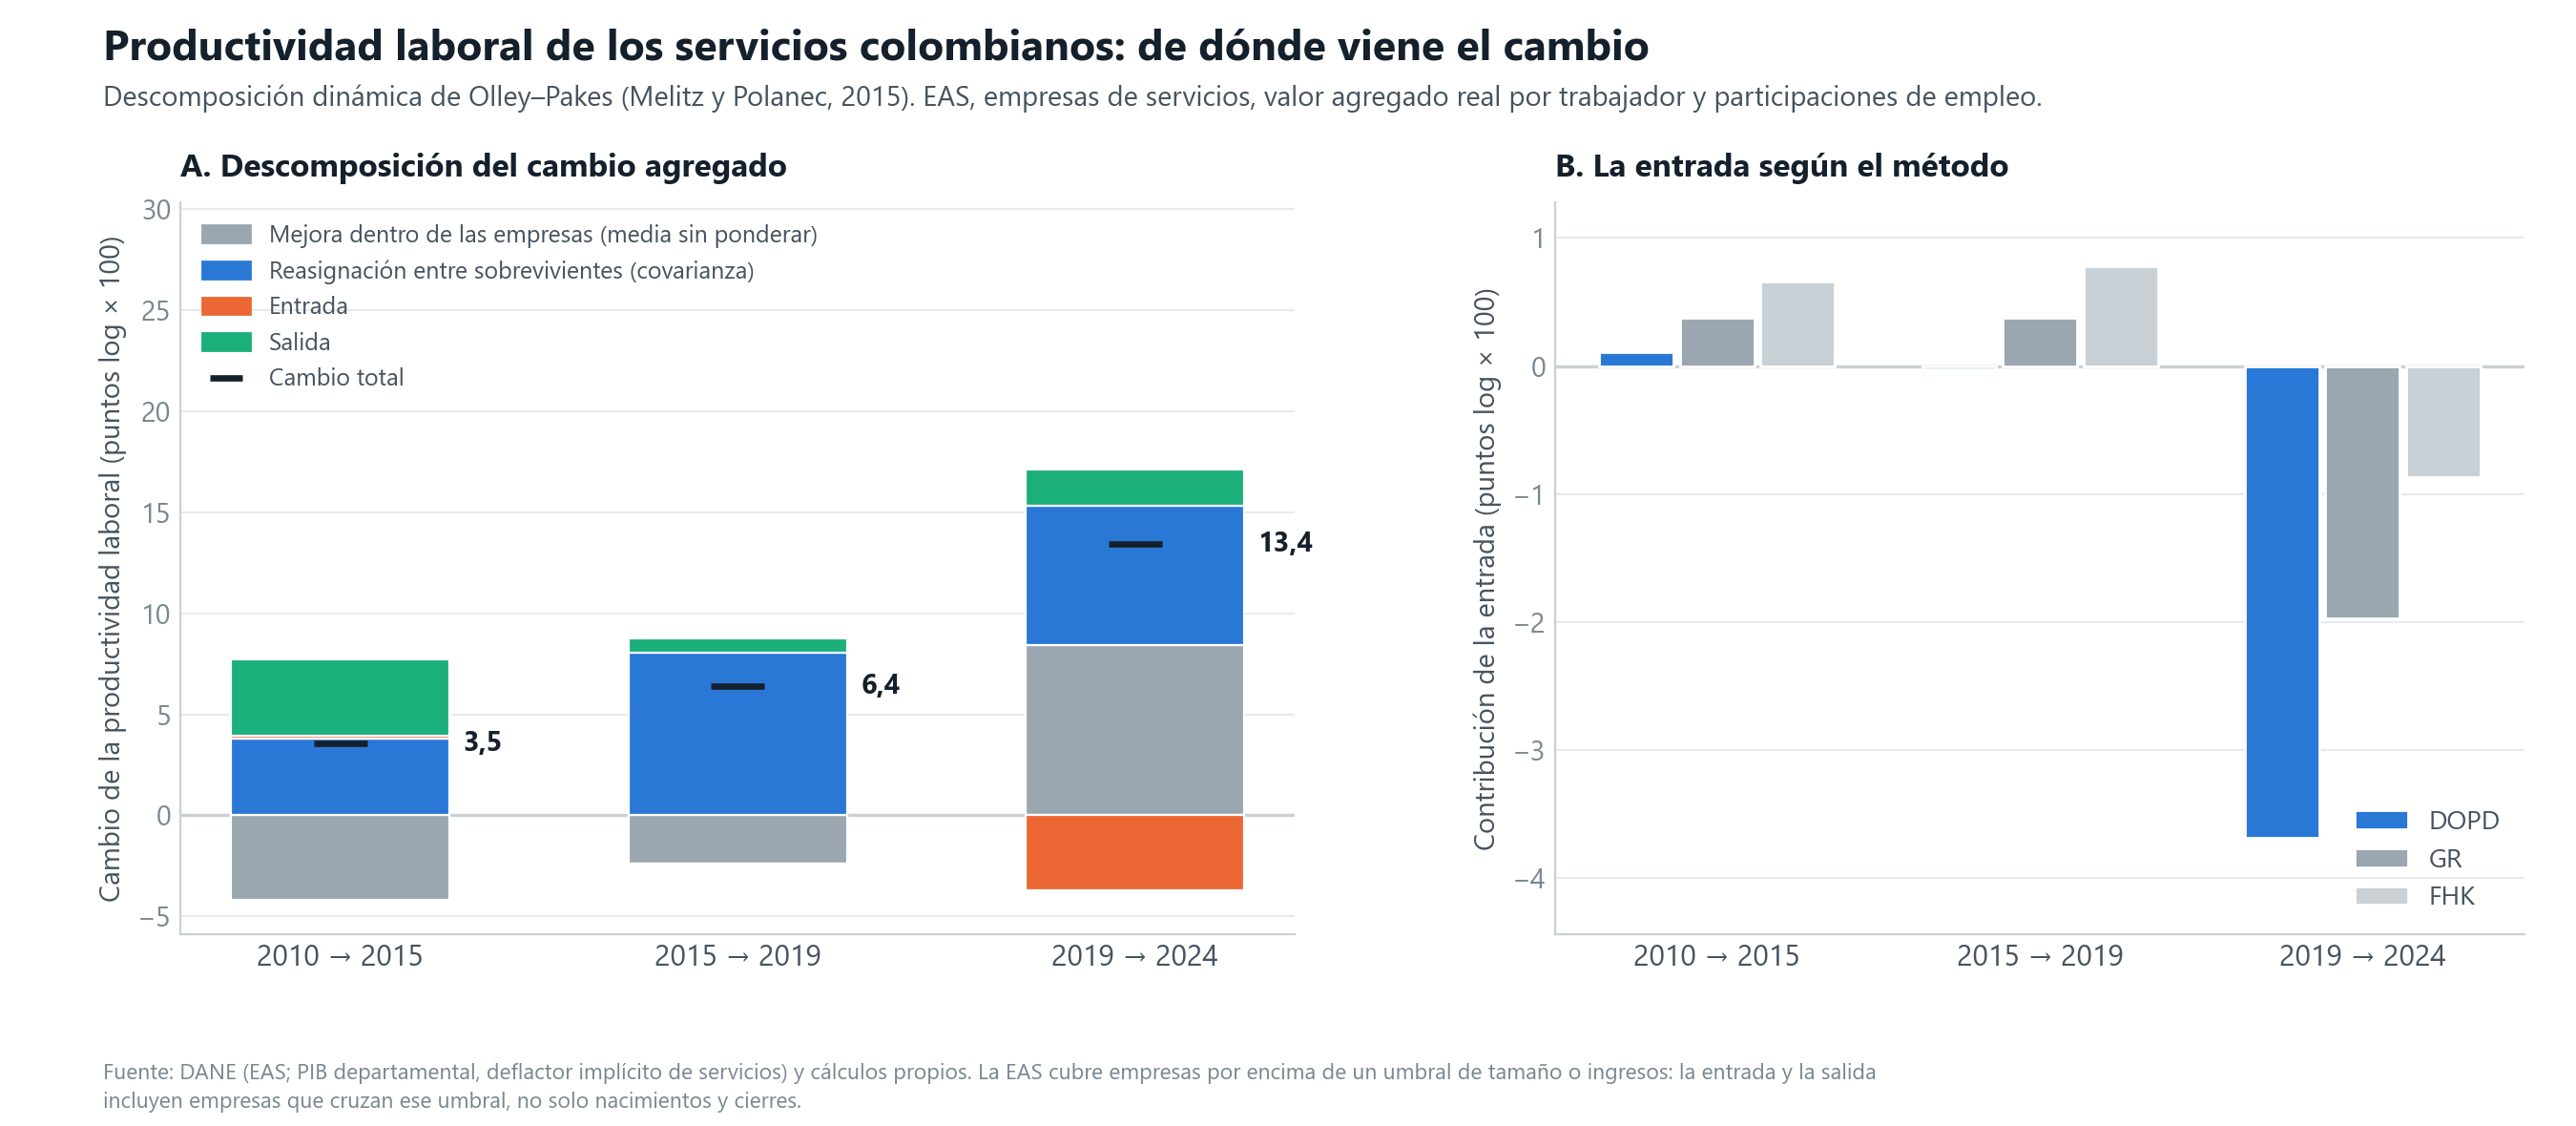
\includegraphics[width=\linewidth]{melitz_polanec/fig_dopd_laboral_EAS.png}
\caption{Servicios: una contribución interna positiva en 2019--2024}
\fuente{Fuente: DANE, EAS y cuentas departamentales; cálculos propios. El universo corresponde a las actividades y empresas cubiertas por la EAS, no a todos los servicios de la economía.}
\end{figure}

La entrada resta 3,7 puntos en 2019--2024, mientras la salida aporta 1,8. La brecha de productividad entre entrantes y sobrevivientes podría reflejar diferencias de tamaño, actividad, maduración o cobertura. La descomposición no permite elegir entre esas explicaciones.

\subsection{Qué sugieren los resultados para la política de productividad}
El patrón industrial invita a investigar las dificultades para elevar la productividad de una base amplia de empresas. El resultado de servicios sugiere estudiar qué actividades explican su mejora reciente. En ambos casos importa entender las condiciones de expansión de las empresas productivas: acceso a financiación, capacidades de gestión, tecnología y mercados son hipótesis que requieren evidencia adicional.

La comparación entre encuestas no permite establecer un ranking sectorial definitivo: difieren las coberturas, los deflactores y, en comercio, el año inicial. Tampoco mide bienestar, calidad del empleo ni el costo social de la salida. El siguiente paso es comprobar la estabilidad de los resultados antes de vincularlos con recomendaciones específicas.
\clearpage
\section{Resultados comparados}
\begin{table}[H]
\centering\small
\caption{Contribuciones al cambio acumulado del índice empresarial}
\begin{tabular}{llrrrrr}
\toprule
Encuesta & Periodo & Total & Media & Cov. & Entrada & Salida \\
\midrule
EAM & 2010--2015 & 8,2 & -0,4 & 6,4 & -1,3 & 3,6 \\
EAM & 2015--2019 & 10,7 & -6,4 & 12,1 & -0,5 & 5,5 \\
EAM & 2019--2024 & 10,4 & -0,1 & 7,5 & -0,7 & 3,8 \\
EAC & 2015--2019 & -0,9 & -10,9 & 7,8 & -0,4 & 2,7 \\
EAC & 2020--2024 & 8,7 & 1,8 & 2,5 & 0,5 & 3,9 \\
EAS & 2010--2015 & 3,5 & -4,2 & 3,8 & 0,1 & 3,8 \\
EAS & 2015--2019 & 6,4 & -2,4 & 8,0 & 0,0 & 0,7 \\
EAS & 2019--2024 & 13,4 & 8,4 & 6,9 & -3,7 & 1,8 \\
\bottomrule
\end{tabular}

\fuente{Fuente: cálculos propios con EAM, EAC y EAS. Puntos logarítmicos multiplicados por 100; puede haber diferencias de suma por redondeo. ``Media'' y ``Cov.'' se calculan entre sobrevivientes.}
\end{table}
Las contribuciones se suman dentro de cada fila. Por ejemplo, un aporte de reasignación superior al cambio total no es un error: puede compensar contribuciones negativas de otros componentes. Al trabajar con logaritmos empresariales, los valores no deben presentarse como el crecimiento porcentual exacto del cociente entre valor agregado total y empleo total.

\subsection{Pruebas pendientes antes de una versión publicable}
Se evaluará si el resultado persiste al excluir extremos de productividad, restringir la muestra a un tamaño mínimo comparable y distinguir entradas y salidas persistentes de apariciones transitorias. En industria se contrastará empresa frente a establecimiento. También se sustituirán los deflactores comunes por alternativas por rama cuando la cobertura temporal lo permita.

En comercio, las prioridades son validar la corrección de variables de 2017--2018 y explorar un puente de identificadores entre 2019 y 2020, sin tratar una coincidencia aproximada como identificación confirmada. Estas comprobaciones deben preceder a cualquier comparación homogénea de los tres sectores.
\clearpage
